%##################################################
\frame{
\frametitle{Email- und Kalenderanbindung}
	\begin{block}{Kommunikation mit Hochschul-Content}
		\begin{itemize}
			\item Hochschul-interne Daten über Content System für Kalender und Email
			\item Content-Zugriff und Update bei Internetzugriff des Mobilfunktgeräts
		\end{itemize}

	 \begin{minipage}{0.6\linewidth}
  		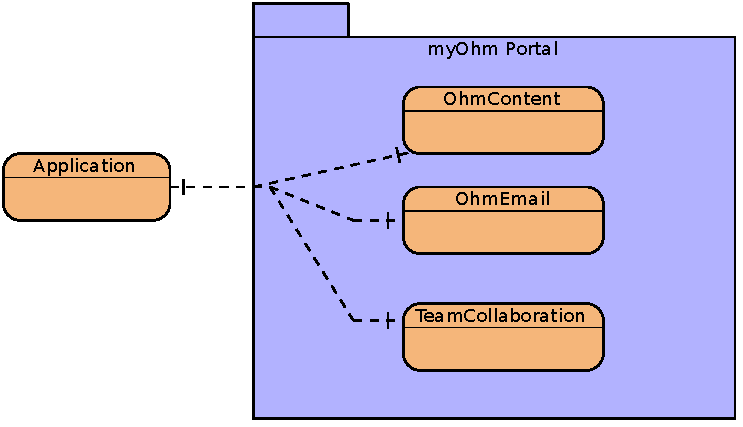
\includegraphics[width=0.9\textwidth]{../grafiken/OhmCollab.pdf}
    \end{minipage}
    \begin{minipage}{0.38\linewidth}
        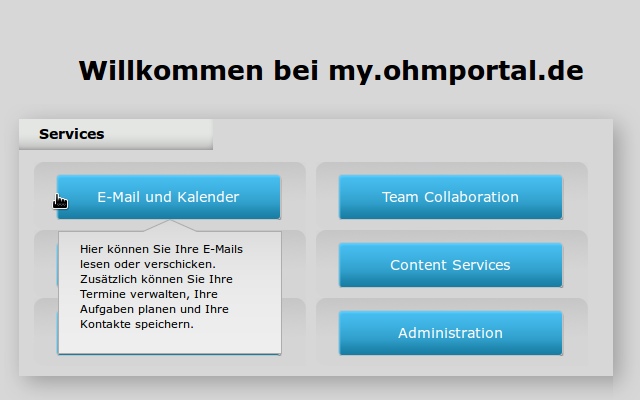
\includegraphics[width=1.0\textwidth]{../grafiken/myOhm.png}
    \end{minipage}
    	\end{block}
}


\frame{
\frametitle{Datenhaltung}
	\begin{block} {Content Management System (CMS)}
	\begin{itemize}
		\item CMS zum Verwalten von Inhalten
		\item Verschiedene Benutzerrollen:	
			\begin{itemize}
				\item Administrator: Bearbeitung von Design und Inhalt
				\item Redakteuer: Bearbeitung von Inhalt
			\end{itemize}
		\item $\rightarrow$ Hochschule benutzt bereits CMS Systeme für Inhalte der Webseite. \\\textbf{Vorteil: zusätzliche Schulung nicht notwendig} 
	\end{itemize}
	\end{block}
	\begin{block}{Diagramm}
		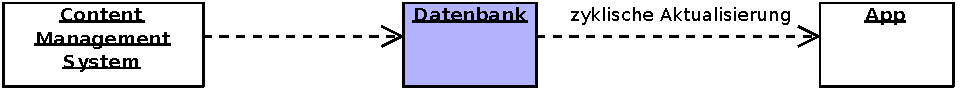
\includegraphics[width=1.0\textwidth]{../grafiken/DB.pdf}
	\end{block}
}


